%*******************************************************************
%   Project Name: BracU Thesis Template
%   Prepared by: Ayesha Abed Library, Brac University
%   
%   "Predicting a T20 Cricket Match Result While The Match is in Progress", this thesis was 
%   submitted to BracU on 23 August, 2015 by Fahad Munir, Md. Kamrul Hasan, Sakib Ahmed, Sultan Md. Quraish
%   Authors have given full consent to use their thesis as a sample to develop a Thesis Template using LaTex 
%   PLEASE KEEP ALL FILES IN THEIR DESIGNATED FOLDERS
%*******************************************************************
% Project Structure:
% appendix: Contains “appendix.txt” files.
% bibliography: Contains “references.bib” file.
% chapters: Contains “chapter.txt” files. For every chapter, create separate “chapter_[1,2,3..].txt” files.
% core: This folder will contain following files:
%     declaration.txt
%     approval.txt
%     ethics_statement.txt
%     abstract.txt
%     dedication.txt
%     acknowledgement.txt
%     titlepage.txt
% images:Contains all images files. 
% main.txt
%     This is the main.txt file. All the packages and environment variable are declared in main.txt. All others .txt files are referred from this file.
%
% If you have any questions or concerns about the latex template, please feel free to visit Ayesha Abed Library.
%*******************************************************************

\documentclass[Times,12pt,oneside,openany,print,index]{report}
\usepackage[a4paper,width=150mm,top=25mm,bottom=25mm]{geometry}
\usepackage[english]{babel}
\usepackage[utf8]{inputenc}
\usepackage{csquotes} % Provides advanced facilities for in-line and display quotations
\usepackage{amsmath} % TO use mathematical equations 
\pagestyle{plain} % Just a plain page number. For more http://www.emerson.emory.edu/services/latex/latex_129.html

\usepackage{graphicx} % to use the graphicx package
\graphicspath{/images} % Path to Image files 
\usepackage{caption} % To use caption with figure and images
\usepackage{array} % The array environment is used to make a table of information, with column alignment (left, center, or right) and optional vertical lines separating the columns

\usepackage[nottoc]{tocbibind} % The tocbibind package can be used to add the ToC and/or bibliography and/or the index etc., to the Table of Contents listing

\usepackage[normalem]{ulem} % The ulem package provides various types of underlining that can stretch between words and be broken across lines.

\usepackage{hyperref} % Provides LaTeX the ability to create hyperlinks within the document.
\hypersetup{
    colorlinks=true,
    linkcolor=black,
    filecolor=magenta,      
    urlcolor=black,
    citecolor=black,
}
\urlstyle{same}

\setlength{\parindent}{0em} % To control Indentation of paragraphs 

\usepackage{nomencl} % The nomenclature package can be used to generate and format a nomenclature using MakeIndex.
\renewcommand{\nompreamble}{The next list describes several symbols \& abbreviation that will be later used within the body of the document}
\makenomenclature

\usepackage[backend=biber,style=ieee,sorting=ynt]{biblatex} % for more plz click https://www.overleaf.com/learn/latex/Biblatex_citation_styles
\addbibresource{bibliography/references.bib} % Imports bibliography file

\let\cleardoublepage=\clearpage % removes unwanted doublepages

\begin{document}

\thispagestyle{empty} % removes page number from title page
\begin{titlepage}
\renewcommand*{\thepage}{Title} % Change page number in PDF

    \begin{center} 
        \vspace*{3cm} % For creating Vertical Blank Space
        
        {\fontsize{17.28pt}{22pt}\selectfont{AUDIO CLASSIFICATION
        }
        } % "fontsize{font size}{line space}\selectfont{}" command to override font size and line space for the Title
        
        \vspace{1.5cm}
        
        \text{by}
        
        \vspace{0.5cm}
        
        MD. Sadman Sakib\\
        18301061\\
        MD. Sakib Hossain\\
        18101201\\
        Syed Tamzidul Islam\\
        18301067\\
        Sujat Mazumder\\
        18101300\\
        Ali Imran Joy\\
        18301179


        \vspace{1.5cm}
        
        	A thesis submitted to the Department of Computer Science and Engineering\\
            in partial fulfillment of the requirements for the degree of\\
            B.Sc. in Computer Science

        
        \vspace{2.5cm}
        
    		Department of Computer Science and Engineering\\
            Brac University\\
            September 2022
        
        \vspace{3cm}
        
    		\copyright\ 2022. Brac University\\
            All rights reserved.
    
    \end{center}

\end{titlepage} % Add title page
\cleardoublepage

\pagenumbering{roman} % Roman numbers to be use all pages before Chapter 1

%*******************************************************************
% TOC = Table of Contents
% The hyperref makes Title page No. 1 entry in the TOC
% In order to properly link  all section in TOC "phantomsection" command used
%  see below link for details on "addcontentsline"
% http://www.emerson.emory.edu/services/latex/latex_162.html
% "input" command to add files
% "Ethics Statement" & "Dedication" page are Optional; you may omit this two page if you want
% Please do not change the order of listings in TOC
%*******************************************************************
\phantomsection
\addcontentsline{toc}{chapter}{Declaration}
% Following command is used to created grouped signature line for Four Authors
\newcommand*\wildcard[2][6cm]{\vspace{2cm}\parbox{#1}{\hrulefill\par#2}} 

% A "parbox{}{}" is a box whose contents are created in paragraph mode. 
% "hrulefill{} to chance thickness of underline"

\section*{Declaration}

It is hereby declared that,

\begin{enumerate} % begin{enumerate} function to create numbered list
  \item The thesis submitted is our own original work while completing degree at Brac University.
  \item The thesis does not contain material previously published or written by a third party, except where this is appropriately cited through full and accurate referencing.
  \item The thesis does not contain material which has been accepted, or submitted, for any other degree or diploma at a university or other institution.
  \item We have acknowledged all main sources of help.
\end{enumerate}

\vspace{1cm}
\textbf{Student’s Full Name \& Signature:} % Testbf{} for Bold

\begingroup

    \begin{center}
        \wildcard{\centerline{MD. Sadman Sakib} ~\\ \centerline{18301061}} % "centerline{}" to center line
        \hspace{2cm} % "hspace{}" for Blank Horizontal space
        \wildcard{\centerline{MD. Sakib Hossain} ~\\ \centerline{18101201} }
        \wildcard{\centerline{Syed Tamzidul Islam} ~\\ \centerline{18301067} }
        \hspace{2cm}
        \wildcard{\centerline{Sujat Mazumder} ~\\ \centerline{18101300} }
        \wildcard{\centerline{Ali Imran Joy} ~\\ \centerline{18301179} }
      \end{center}

\endgroup


\pagebreak







\phantomsection
\addcontentsline{toc}{chapter}{Approval}
\section*{Approval}

The thesis/project titled “AUDIO CLASSIFICATION” submitted by 
\begin{enumerate}
  \item MD. Sadman Sakib (18301061)
  \item MD. Sakib Hossain (18101201)
  \item Syed Tamzidul Islam (18301067) 
  \item Sujat Mazumder (18101300)
  \item Ali Imran Joy (18301179)
\end{enumerate}

Of Spring, 2022 has been accepted as satisfactory in partial fulfillment of the requirement for the degree of B.Sc. in Computer Science on September, 2022. 

\vspace{0.5cm}
\textbf{Examining Committee:}

\vspace{1cm}

Supervisor:\\
(Member)
\begin{center}
    \hspace{7cm} \wildcard{\centerline{Aminul Huq } ~\\ \centerline{Lecturer}~\\ \centerline{Department of Computer Science and Engineering}~\\ \centerline{BRAC University} } \hspace{1cm} 
\end{center}

Program Coordinator:\\
(Member)
\begin{center}
    \hspace{7cm} \wildcard{\centerline{Name of Program Coordinator} ~\\ \centerline{Designation}~\\ \centerline{Department}~\\ \centerline{Brac University} } \hspace{1cm} 
\end{center}

Head of Department:\\
(Chair)
\begin{center}
    \hspace{7cm} \wildcard{\centerline{Name of Head of Department} ~\\ \centerline{Designation}~\\ \centerline{Department of Computer Science and Engineering }~\\ \centerline{Brac University} } \hspace{1cm} 
\end{center}

\pagebreak


\phantomsection
\addcontentsline{toc}{chapter}{Abstract}
\section*{Abstract}
Sounds have a wealth of information that enhances our understanding in this unprejudiced world. 
Every day we face many sounds around us. From this sound we filter all sounds in our brain cell and provide with a result what sounds are fit in which dice. 
For this not only our brain cells many machines are also available. Working with sound classifications, can improve recommendations in various applications. To work properly these machines, need to know the right way to extract data from it. Digital audio has a lack of structured organizations. So that it brings significant complexity to sound classification work. Keeping that in mind we intended to do research in sound classification. The primary goal of our research is to find which feature fits our model and gives us maximum values that we desire for. All the while we will try to analyze different models to see which work more efficiently. Our plan is to collect speech command dataset from online sources. We intended to use deep learning methods to analyze our data in different features. Those features are MFCC, Mel Spectrogram, Wavelet. For our model we use conventional neural networks (CNN), long short-term memory (LTSM). Also, we will analyze raw data without implementing any features. 




\vspace{1cm}
\textbf{Keywords:}  convolutional neural networks (CNN), LSTM, Deep learning, Mel Frequency Cepstral Coefficient (MFCC), Wavelet. Mel-Spectrogram.
\pagebreak


\phantomsection
\addcontentsline{toc}{chapter}{Acknowledgment}
\section*{Acknowledgement}
Firstly, all praise to the Great Allah for whom our thesis have been completed without any major interruption.\\
Secondly, to our beloved Aminul Huq sir and Rafeed Rahman sir, for their kind support and advice in our work. They helped us whenever we needed help.\\
And finally to our parents, without their throughout support it may not be possible. With their kind support and prayer, we are now on the verge of our graduation.

\renewcommand{\contentsname}{Table of Contents} % Rename TOC name from Contents to Table of Contents
\cleardoublepage
\phantomsection
\addcontentsline{toc}{chapter}{Table of Contents} % Add Table of Contents in TOC
\tableofcontents % To  generation of the Table of Contents



\pagenumbering{arabic} % To use page number 1,2,3 ..

\chapter{Introduction}
%\section{Introduction}
\section{Audio Classification} 
Audio classification is an expanding field of research with several real-world applications. Recent advances in image classification, where convolutional neural networks are used to classify pictures with high accuracy and at scale, raises the issue of whether similar approaches may be applied to other domains, such as audio classification. Audio classification or sound classification is the process of analyzing audio recordings and categorizing them in a proper way. Basically, audio classification is the task of assigning a label or class to a given audio. It may be used to identify a speaker as well as recognize which command a user is issuing or the mood of a speech. Audio classification can be of multiple types and forms such as-Acoustic event detection, music classification, Natural language classification and environmental sound classification. Despite recent advances in the field of audio classification, teaching a machine to recognize a sound and classify it into several categories is a tedious process. Starting with annotated audio data is the initial step in solving audio categorization challenges. Here are several relevant datasets for various sorts of sounds. These datasets contain a huge number of audio samples, as well as a class label for each sample that indicates what sort of sound it is, depending on the problem we’re attempting to solve. The automated classification of audio is a major challenge. Several authors have proposed methods to categorize incoming audio data based on different techniques throughout the previous decade. The majority of the proposed systems incorporate two phases of processing. The first stage analyzes the incoming waveform and extracts certain features from it. The feature extraction process generally entails a significant amount of data reduction. The second stage performs a classification based on the extracted features. A variety of signal features have been proposed for general audio classification. A second important feature set which is inherited from automatic speech recognizers consists of mel-frequency cepstral coefficients (MFCC). We applied Convolutional Neural Network (CNN) and Recurrent Neural Network (RNN) along with MFCC to improve the work proficiency of our model and tried to make comparisons with other models. CNN has shown to be effective in voice classification. We’ll exhibit how to apply Deep 4 Learning techniques to the classification of audio, specially focusing on the identification of particular sounds.
\section{Problem Statement}
Nowadays in the current world, speech recognition has gained prominence and use with the rise of AI and intelligent assistants, such as Amazon Alexa, Apple Siri, Microsoft Cortana, Google assistant. Speech recognition is the ability of a machine or a program to identify words and phrases in spoken language and convert them to a machine-readable format. Speech recognition has many applications such as voice dialing, call routing, search keywords, simple data entry. Today in the current generation speech recognition is playing a major role in most of the fields such as smartphones, Tv, voice call routing, voice dialing, search keywords, simple data entry. We all know that whenever we call any customer care service there will be a virtual assistant to assist us before we reach the main person to whom we want to talk. The technique used here was Call routing which refers to the procedure of sending voice calls to a specific queue based on predetermined criteria. A call routing system is also known as an automatic call distributor (ACD). Since traditional models of customer service were based on phone support or call support as one of the primary methods of contact between customers and companies for business purposes, the procedure of sending calls to the right agent became very much important. Today, modern agents interact with customers through a variety of channels. In earlier days most of the people use to call by typing the number in the phone but nowadays voice-enabled calling is also available where people use to call anyone through their voice without typing any number in the phone, this has made easier to the people but the problem is if anyone is in such a place where there is more noise and more disturbance then voice-enabled calling may not work correctly as more than two or more voices mixes, where it will be difficult for a system to recognize our voice in such a worst environment. To overcome this best noise elimination technique should be used where it can eliminate noise up to a level. Voice enabled calling is also known as voice dialing which uses speech recognition software. In the present world, it is possible to entry some of the data in excel or word documents using our voice which enables you 6 to do hands-free data entry by dictating the text or numbers that we want to be entered in the current cell and to issue voice commands that allow you to choose menu items, dialog box options, or even toolbar buttons by simply saying their names. This saves our time and work can be done faster compared to typing work. Even for voice data entry speech recognition software has been used. When using Speech Recognition to dictate data entries, we need to keep the microphone close to our mouth and in the same position as you dictate. Depending upon the microphone quality we need to speak normally and in a low but not monotone voice, pausing only when you come to the end of a thought or the data entry for that cell and it takes time for our computer to process our speech, and therefore, depending upon the speed of your processor, it may take some time before your words appear on the Formula bar and in the current cell. This can be improved by training more and more audio data using deep learning or machine learning algorithms. As we know Google Assistant and Microsoft Cortana are widely used nowadays such as searching for information on the internet or it may search for information on the computer such as files, folders, documents, and many other things. All these are done through our voice, whatever we speak, or we tell Google Assistant and Microsoft Cortana it will search and give us a piece of information about what we require. Therefore, Speech recognition is playing a major role in Google assistant, Microsoft Cortana, and Apple Siri. Day by Day the accuracy of converting from speech to text in Google Assistant, Microsoft Cortana, and Apple Siri is increasing. Think of a situation where you want to share your feelings to someone or you want someone to entertain you in your sad times then Amazon Alexa or amazon echo can be used, whenever we speak it will listen to us and give some information like if we tell "Alexa sing a song" it will sing some song for us or if we tell "Alexa tell us some news about today" so Alexa will tell us the news about today, Amazon Alexa is speech recognition device which recognizes our speech and depending upon that it gives some output.
\section{Research Objective }
In our research, we proposed an efficient way to classify audio data of different objects using deep learning methods using neural networks. Here, we aim to prepare a deep learning model that can predict the accuracy of different models through extracting features from the Speech Command dataset. Our prior objective is to determine the wav files so that the devices whose work is based on voice can predict properly and give better results by fulfilling customer requirements. The remaining objective is as follows:
 
•	Organizing Audio library for each class.\\
•	Finding the best performance algorithms which can work more precisely on different scenarios. \\ 
•	By using different feature extraction techniques to analyze music genre identification.\\
•	Finding different audio pattern using deep neural network 


\chapter{Litareture Review}

MFCC and Chroma STFT \parencite{1} stack together features which are used in LTSM model are giving state-of-the-art result. In our world we are surrounded with many sounds which is not possible to process all by our brain cell. Thats why many research field are work on sound classification for many purposes such as audio surveillance, multimedia and many more. so, as said before there are many features that are used in this paper. Those are mel spectrogram, spectral contrast, tonnetz, MFCC, Chroma CENS and Chroma CQT. From models there are used CNN and LSTM.There are lots of other papers that are used in this paper for better performance. In dataset is shows deep learning models are performing better performance then machine learning models. The audio samples were in wave from but it was converted into a one-dimensional NumPy array of digital values. There was a librosa package used for normalizing so that values can be represented in the array. Also works as time stretch and pitch shifting. After implementing all spectrograms in CNN and LSTM it shows MFCC was best features. Where stacking MFCC and Chroma STFT helps to reach validation accuracy of 98.81\% where best performance was 98.60\%. Also, LTSM does a better job because LSTM memory cell includes constant error backpropagation which deals with data noise. 

Cardiovascular diseases have leading cause of mortality rate where, Wavelet representations and RNN \parencite{2} can be used for recognizing three heart sounds i.e., normal, mild, severe. This works needs physicians who are trained also approx. 20\%of the medical interns on average can use efficient use of stereoscope to measure subjects’ heartbeat. There are some limitations in work such as publicly accessible data, deep learning methods are not 8 comprehensively studied. In the experiment coif3 was selected for wavelet type. DRNN model was optimized to have three layers with adam optimizer. So, in results wavelet based DRNN works excellent performance in reckoning mild class. The value of normal and severe can be improved. This is hard for this model to distinguish between these three models. 

Machine learning advances have sparked renewed interest \parencite{3} in a variety of classification challenges, particularly those incorporating data in the form of photos, videos, and audio recordings. Classifying sounds and predicting their category is one of the most common classification challenges. Security systems, classifying music clips to identify the genre of the song, classifying distinct surrounding sounds, speaker recognition, and verification are some of the real-world uses for such a classification model. The task of assessing diverse audio signals is known as audio classification. They gave a brief overview of the field of audio classification in this work, describing the system, several modules of feature extraction and modeling, applications, underlying approaches, and certain performance indicators. Following this introduction, we'll go over some of the present classification technologies' strengths and drawbacks, as well as some prospective future research, development, and application trends. Many audio classification subtasks rely heavily on inputs, network topologies, temporal pooling strategies, and objective functions, so we paid special attention to them. Finally, the study discusses future trends and research prospects in this field.

A novel audio finger methodology  for audio classification is proposed in this research. The audio signal's fingerprint is a unique digest that can be used to identify it. To establish a unique fingerprint of the audio files, the suggested model employs the audio fingerprinting methodology. The fingerprints are made by 9 extracting an MFCC spectrum, taking the mean of the spectra, and then converting the spectrum to a binary picture. These images are then sent into the LSTM network, which classifies the environmental noises included in the UrbanSound8K dataset with an accuracy of 98.8 \% across all 10 folds. 

It is critical to provide security for women and children in light of increased crime against them. Several contemporary techniques Nowadays, they're employed to provide security. Some of them are sensor-based gadgets \parencite{5}, while others are mobile apps. But When sensors are present, hardware-based gadgets do not function properly and are cut off from their bodies Existing applications on the Mobile gadgets are not always functional. Victims must take action. Specific reactions such as shaking the phone and pressing the SOS button, which may or may not be available at all times. As audio one of the most advanced applications of deep learning is classification. They presented an idea to provide protection for women and children through learning. Audio classification is used by youngsters. The victim's screaming sounds, which can be heard from quite a distance, have alerted them of danger. For audio classification, a few deep neural network models are used, so various audio and reaction screams can be considered a sign of danger. They've also created a new dataset specifically for this. 

A novel strategy for dealing with the presence of unseen sound classes (open set) and the scarcity of training resources \parencite{6} while deploying audio classification systems in operations is proposed, which incorporates variational auto-encoder (VAE), data augmentation, and detection-classification combined training into standard GAN networks. The VAE input to GAN-generator aids in the generation of realistic outlier samples that are not too distant from the in-distribution class, hence improving classifiers' open-set discriminating capabilities. The augmentation enhanced GAN scheme developed in their previous work for close-set audio classification will then help to address the limited training resources by combining physical data 10 augmentation with traditional GAN produced samples to avoid overfitting and improve optimization convergences. The detection-classification joint training builds on the advantages of VAE and Augmentation GAN to improve detection and classification task performance. Experiments using the Google Speech Command database indicate significant increases in open set classification accuracy from 62.41 percent to 88.29 percent when only 10\% of the training data is used. 

A Deep Belief Network (DBN)-based technique \parencite{7} for audio signal classification is proposed to improve labor activity identification and remote construction project surveillance. The goal of this project is to provide an accurate and adaptable platform for performing and controlling unmanned construction site monitoring utilizing distributed sound sensors. To perform and validate the proposed approach, 10 classes of numerous construction equipment and tools, often and widely used on construction sites, were collected and examined in this study. The DBN receives a concatenation of multiple statistics evaluated by a set of spectral features, such as MFCCs and mel-scaled spectrograms. The proposed architecture, as well as the preprocessing and feature extraction stages, have been thoroughly defined, and the usefulness of the proposed concept has been shown by numerical results based on real-world recordings. The final total accuracy on the test set was up to 98 percent, which is much better than other state-of-the-art methodologies. In order to apply the categorization scheme to sound data acquired in various environmental settings, a practical and real-time application of the presented method has also been proposed. 

Sound files for Animal sound classification using deep learning and CNN architecture, were preprocessed \parencite{8} in such a way that it can extract MFCC using librosa. There are also some studies that show that with a limited dataset CNN using log MEL-spectrogram performs best with 64.5 accuracy. 11 The data was collected online in WAV format and these are used in 3 different ways. First, they examine all manually to prevent low quality sound. Secondly all are WAV format because MFCC supports WAV format in feature extraction. Thirdly, the size of the sound file was 3 kilobytes. By using Librosa all dataset were preprocessed as binary files for Training and Testing. For activation functions it used Relu. For testing it takes 80\% of data and for training it takes 20\% data and finally it shows 75\% accuracy by Nesterov-accelerated adaptive moment estimation. 

Urban sound classifications have multiple features, which are implicated on different neural networks to see which model gives better accuracy in classifying audio signals. In our world we are surrounded with many sounds which are not possible to process all by our brain cells. That's why many research fields work on sound classification for many purposes such as audio surveillance, multimedia and many more. so, as said before, there are many features that are used in this paper. Those are mel spectrogram, spectral contrast,tonnetz,MFCC,Chroma CENS and Chroma CQT. From models there are CNN and LSTM.There are lots of other papers that are used in this paper for better performance. In dataset it shows deep learning models are performing better performance then machine learning models. The audio samples were in wave form but they were converted into a one-dimensional NumPy array of digital values. There was a librosa package used for normalizing so that values can be represented in the array. Also works as time stretch and pitch shifting. After implementing all spectrograms in CNN and LSTM it shows MFCC has the best features. Where stacking MFCC and Chroma STFT helps to reach validation accuracy of 98.81\% where best performance was 98.60\%. Also, LTSM does a better job because LTSM memory cell includes constant error back propagation which deals with data noise. So, lastly this paper shows that using MFCC and Chroma STFT stack together features which are used in the LTSM model are giving state-of-the-art results.

CNN is a good way to implement in Environmental sound classifications \parencite{12}. For this CNN there are some steps that were followed in this paper. All the data are labeled for efficient learning. There were multiple datasets used (ECS-50, ECS-10). After implementing it in CNN it shows better results even with a limited dataset. When the dataset number will increase it will perform more accurately in the environmental dataset. Speaking Faces is made up of synchronized audio, thermal, and visual data collected from a wide range of people. They used their data to do thermal-to-visible image translation and multimodal gender classification using thermal, visual, and auditory data streams to illustrate its applicability. They saw that Speaking Faces has the following good effects based on the experimental results. For starters, it allows for more in-depth research into multimodal recognition systems that use optical, thermal, and aural modalities. Second, the enormous number of samples in the dataset makes it possible to build and test data-hungry neural network techniques. Finally, synced multimodal data can offer up new avenues for domain transfer study. They intend to use our dataset for more multimodal tasks in the future, such as audio–visual–thermal speech and speaker recognition. By leveraging 150 hours of OOD data and adjusting with 5 hours of in-domain transcribed data, SR models for controller pilot communication for the Vienna approach were developed. To take use of inexpensively available untranscribed in-domain data, we suggested data selection algorithms based on word and concept level confidences. This was used to supplement transcribed in-domain data, allowing both acoustic and language models to be adjusted. When compared to using only in-domain transcribed data (ASR- DEV1, WER: 12.3 percent, CER: 38.6 percent), using OOD data and complementing transcribed data with untranscribed in-domain data through data selection reduces WER by 23.5 \% (using word confidences) and CER by 7\% (using concept confidences). We will investigate using larger volumes of untranscribed data in the future. 

A hybrid classical-to-quantum transfer learning method \parencite{13} for QNNs can be used in SCR where, CNN-QNN-based SCR system after setting up the VQC-based QNN. A pre-trained CNN framework is transferred to a hybrid transfer learning framework.so that we might improve the performance of CNN-QNN system Using the Google speech command dataset, found that, the importance of hybrid classical-to-quantum transfer learning in improving classification precision and reducing cross-entropy loss the CNN-QNN model's value. 
A smart home system \parencite{10} saves time and energy, especially when a large number of people are involved. A large number of people are involved. It might be expanded to include video surveillance to detect persons in crowded places like bus stops, theaters, and train stations, where the perpetrator's identity can be verified. Face recognition techniques are used. In the field of computer vision, the recognition system is a challenging matter to tackle. Due to its wide uses in a variety of sectors, it has recently sparked a lot of attention. Despite extensive efforts, Research efforts in this field have yielded robust facial recognition systems that can work in a variety of environments. They are still far from fulfilling the ideal of being able to perform well in limited spaces. 

Door Access Control System \parencite{11} only enables those who have an approved key card and whose voice has been recorded in the system. The technology of voice recognition recognizes your voice and the words you say. Because your voice cannot be stolen, it is a safe way to prevent illicit admission into an organization. If you're experiencing difficulty speaking, An RFID-enabled key card can be utilized (probably sick). As a prototype, the work was successful, and the prototype was successful. 14 The door was able to unlock when the user spoke into the microphone or swiped the RFID card. This is the first version. Further improvements to this work can be done before. 

Adversarial attacks \parencite{12} are the biggest threat to speech recognition, especially for Deep Learning-based systems. Some researchers have created adversarial speech examples for speech recognition based on FGSM. Genetic algorithms have also been used to fool speech recognition systems into saying that all is well. In this paper, they investigate the effectiveness of adversarial attacks on speech recognition components for mission-critical applications and provide defense techniques against adversarial attacks. They also outline the challenges and directions for future research as well as outline the current state of the art in speech recognition. Speech recognition provides a natural interface for human communication. It allows machines to process human voice and to generate a text transcription. Integrating voice recognition with conversational systems opens the door for incredible potential in many real-world applications. There are different methods for feature extraction such as Mel Frequency Cepstral Coefficients (MFCC), Perceptual Linear Prediction (PLP), linear predictive coding (LPC), Discrete wavelet transform (DWT), Linear prediction cepstral coefficient (LPCC), Fast Fourier Transform (FFT), and Line spectral frequencies (LSF). The aim of the decoding step is to convert an input audio into words by searching the most likely sequence. This task is mainly carried out by learning algorithms such as Hidden Markov Models (HMMs using the Viterbi algorithm that limits the number of searches and finds the optimal path in polynomial time) or deep learning. GMM-HMM is a statistical approach to estimate hidden information from visual signals. The decoder in a speech recognition system is modeled as a Markov process with unknown parameters, signified by the known observable parameters. Integrating a Gaussian Mixture Model with Hidden Markov Model outperformed conventional HMM and GMM-based systems. Hybrid DNN-HMM models are the earliest Deep Learning approaches for speech recognition, where a DNN replaces the acoustic module while keeping the remaining modules. The current trend is to build end-to-end speech recognition systems based on DNNs. This approach can resolve the limitation of the traditional system in which the overall system may not be optimal.

\parencite{14} Features are initially extracted from short-time Fourier transform (STFT) spectrograms via a convolutional neural network. The model was trained and tested on the ICBHI 2017 respiratory 16 Sound Database and achieved state-of-the-art results using three different data splitting strategies. Results include sensitivity 47.37, specificity 82.46\%, score 64.92\% and accuracy 73.69\%. Features initially extracted from short-time Fourier transform (STFT) spectrograms via a convolutional neural network (CNN) are given as input to a long short-term memory (LSTM) network that memorizes the temporal dependencies between data and classifies four types of lung sounds, including normal, crackles, wheezes, and both crackles and wheezes. In this paper they proposed a hybrid DL architecture that combines CNN and LSTM. models for the classification of normal and adventitious lung sounds. Training and evaluation of the model are performed on lung sounds, which includes normal sounds as well as three types of adventitious sounds such as crackles and wheezes. In this study, respiratory cycles were transformed into STFT spectrogram\r images and passed through a CNN that is capable of extracting their most significant features. The extracted features were fed into an LSTM that identifies and memorizes long-term dependencies between them.
 
CNN-TT-DNN \parencite{15} model replaces fully connected (FC) layers with TT ones and can substantially reduce the number of model parameters while maintaining the baseline performance of the CNN model. Our experimental results show that the proposed CNN +(TT-DNN) model attains a competitive accuracy of 96.31\% with 4 times fewer model parameters than the CNN model. The entire CNN framework consists of 4 components, each of which is constructed by stacking 1D convolutional layers with batch normalization and the ReLU activation. The spectral features associated with the outputs of the CNN framework are fed into the FC layers or TT layers. We set our baseline system as the CNN+DNN architecture in which several FC layers are stacked on top of the CNN layers. THEIR models are trained with the same SCR dataset from scratch without any data augmentation to make a fair architecture-wise study. We extend the 10 classes training setup used in 35 classes to report its final results. The CNN+(TT) and CNN+(DNN) models are compared with three other neural networks available in the literature. The CNN+DNN model is taken as the baseline SCR system, and attains 94.42 accuracy and 0.251 CE score. It outperforms the DenseNet, neural attention, and QCNN models in terms of smaller model size, lower CE value, and higher classification accuracy. 

TTTD \parencite{16} can maintain and even obtain better results than the primitive models. Baseline models (DenseNet, neural attention, and QCNN models), when the CNN+(TT-DNN) model is initialized randomly or derived from a well-trained CNN+DNN. Tucker decomposition cannot maintain the DNN baseline results as CNN +DNN models. This work investigates the implementation of a low-complexity SCR system by applying the TT technique. A hybrid model, namely, CNN+(TT-DNN), is proposed to realize an end-to-end SCR pipeline. The proposed model can be randomly initiated or derived from a well-trained CNN \+ DNN.

By taking into account trade-offs between the model complexity and actual performance, low complexity hybrid tensor networks [13] are created. Additionally, CNN+(LR-TT-DNN) has many TT layers at the top for problem-solving in regression and classification and convolutional layers at the bottom for feature extraction. First, we use a low-rank tensor-train deep neural network (TT-DNN) to create the LR-TTDNN, a whole deep learning pipeline. The optimization landscape is made simpler by an over-parameterized deep neural network (DNN), which also assures that local optimum points are near the global ones. Numerous novel applications, such as mobile-based audio de-noise and speech recognition systems that operate on users' phones without sending queries to a distant server where a sizable deep learning model is set up, might be made possible by an effective low-complexity speech improvement system. Two methods exist for reducing the size of deep learning models. One involves the adoption of new deep learning architectures, such as convolutional neural network (CNN) with a variety of innovative topologies. Model pruning and sparseness approaches are mentioned in another. The experiments of voice enhancement and spoken command recognition (SCR) systems are shown to demonstrate the usefulness of our suggested models as we study the deployment of low-rank tensor-train (TT) networks. They have created the CNN+TT-DNN, a brand-new deep hybrid tensor-train model. A CNN is at the bottom, and a DNN is at the top. Time-series signals are transformed into the relevant spectral properties using the CNN model. The DNN is used to address regression or classification issues further. To evaluate the empirical performance of the two models, we independently use spoken-recording experiments and speech enhancement. The TT-DNN model obtains a worse MAE score than the DNN model despite having significantly fewer model parameters (0.604Mb vs. 30.425Mb) (0.664 vs. 0.675). With greater PESQ and STOI scores, the hybrid model CNN+DNN may greatly increase the DNN basis. In this study, two brand-new TT models—LR-TT DNN and CNN-TT-DNN—were introduced, and their effectiveness was evaluated using SCR and voice enhancement tasks.


\chapter{Methodology }
\section{Working Process }
The workflow diagram in Figure 3.1 below shows an overview of each step to train, test, and validate our models.\\
 
First of all, we will collect our data sets. Then we will do data preprocessing through scaling, normalization, resizing, and augmentation. After finishing preprocessing, we will split our dataset into an 8:2 ratio. in which 80\% of the data set will be for training our model and 20\% will be for testing. After that, we will be doing feature extraction methods like Mel Spectrogram, MFCCs, and Wavelet. We will also take raw data to analyze our results. Then, through several neural network models like CNN and LSTM, we will train our model. After that, we will do a comparison to find the validation accuracy of our model. From the comparison, we will select some top Neural Network models that will result in the highest accuracy and add them to get more precise results. Finally, we will reach a conclusion based on the results of our model. 
\section{Used Feature Extractions and Architectures  }
    \subsection{Mel Spectrogram}
    The Mel Spectrogram is a visual representation of sound waves in which frequency and intensity are represented by the x-axis and y-axis, respectively. In it, time appears on the x-axis while various frequencies of sound appear on the y-axis. The different colors represent different intensity levels or frequencies of sound. CNN-LSTM achieves an accuracy of 64.58\% with MFCC features and ResNet-LSTM achieves an accuracy of 62.5\% using log-Mel spectrograms \parencite{16}. We took samples of air pressure over time to digitally represent an audio signal. We mapped the audio signal from the time domain to the frequency domain using the fast Fourier transform, and we performed this on overlapping windowed segments of the audio signal. We converted the y-axis (frequency) to a log scale and the color dimension (amplitude) to decibels to form the spectrogram. We mapped the y-axis (frequency) onto the mel scale to form the mel spectrogram. The audio signal goes to framing and transforms through Discrete Fourier. After mel filterbank and log, the audio is extracted and transformed as a Mel Spectrogram. 
            \begin{figure}[ht]
            \centering
            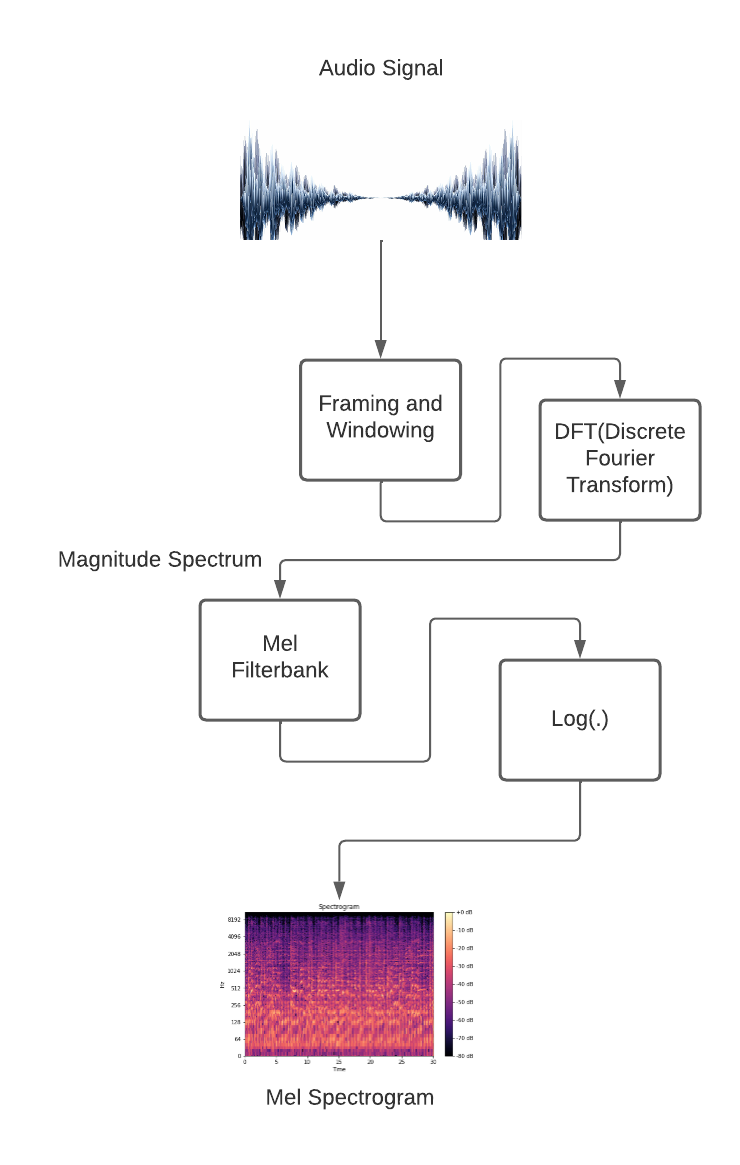
\includegraphics[scale=0.5]{images/figure1.png}
            \caption{Block diagram of Mel spectrogram of an audio signal.}
            \label{fig: Mel Spectrogram}
            \end{figure}
    \subsection{Wavelet}
    The Fourier transform is a useful tool to analyze the frequency components of the signal.  Wavelet transforms are based on small wavelets with limited duration. The translated-version wavelets locate where we concern. Whereas the scaled-version wavelets allow us to analyze the signal in different scale.
    \subsection{MFCC}
    Mel Frequency Cepstral Coefficients (MFCC), The Cepstral coefficients are the inverse-fft of the log of the spectrum; The MFCC are the inverse-fft of the log of the frequency-warped spectrum. The idea of MFCC is to convert audio in time domain into frequency domain so that we can understand all the information present in speech signals. MFCC is to convert time domain signals into frequency domain signal by mimicking cochlea function using Mel filters.
        \begin{figure}[ht]
        \centering
        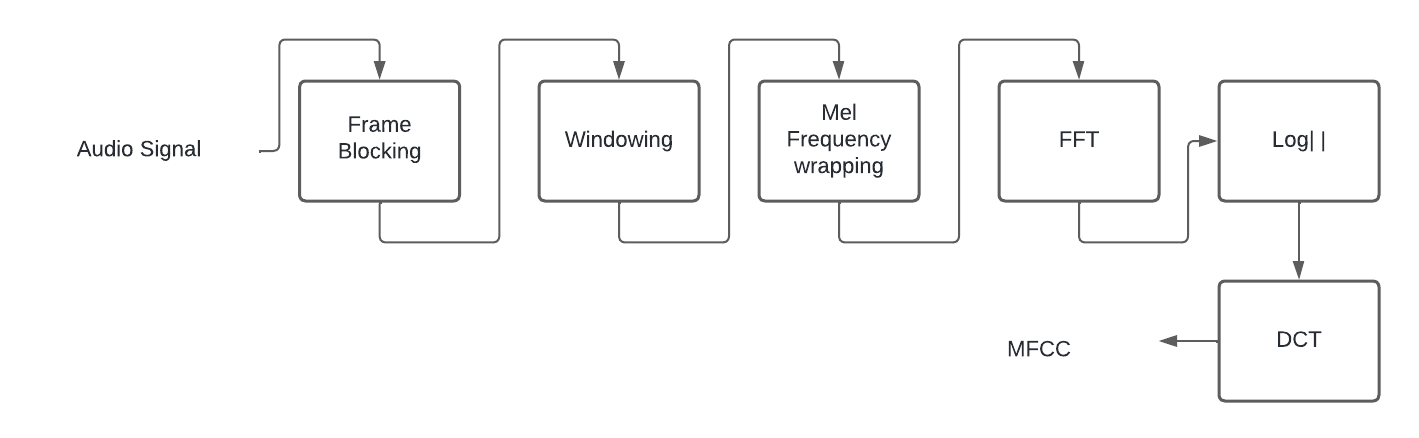
\includegraphics[scale=0.48]{images/figure2.png}
        \caption{Block diagram of MFCC.}
        \label{fig:x Block diagram of MFCC.}
        \end{figure}
    
    \subsection{CNN}
    A convolution tool that separates and identifies the various features of the audio for analysis in a process called "feature extraction." The network of feature extraction consists of many pairs of convolutional or pooling layers. A fully connected layer that utilizes the output from the convolution process and predicts the class of the audio based on the features extracted in previous stages. This CNN model of feature extraction aims to reduce the number of features present in a dataset. It creates new features which summarize the existing features contained in an original set of features. There are many CNN layers, as shown in the CNN architecture diagram.
    \begin{figure}[ht]
        \centering
        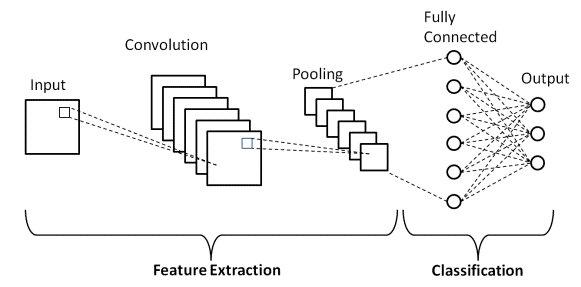
\includegraphics[scale=1]{images/figure3.png}
        \caption{Block diagram of CNN.}
        \label{fig:x Block diagram of CNN.}
        \end{figure}
    \subsection{LSTM}
    Aside from singular data points like photos, LSTM has feedback connections, making it capable of processing the complete sequence of data. This has uses in machine translation and speech recognition, among others. A unique version of RNN called LSTM exhibits exceptional performance on a wide range of issues.


\chapter{Implementation  }
\section{Dataset }
Our dataset consists of 105841 .wav files in 41 folders in random order. 

\subsection{Source }
Pytorch Speechcommand dataset Link: \\
(\url {https://pytorch.org/audio/stable/datasets.html#speechcommands})
\subsection{Data Sample  }
The data set samples are elaborated as follows:
    \begin{figure}[ht]
            \centering
            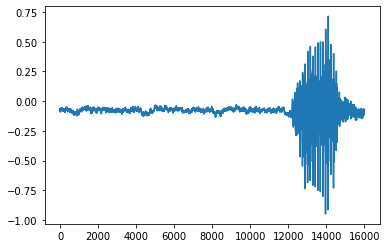
\includegraphics[scale=1]{images/figure4.png}
            \caption{Block diagram of Mel spectrogram of an audio signal.}
            \label{fig: Block diagram of Mel spectrogram of an audio signal}
            \end{figure}
We can comprehend two things after looking at the waveform and the label. Since the labels are text, we must first translate them into class numbers. Second, we confirm that each data sample, or 1x16000, is the same length.            
\section{Data Preprocessing }
\subsection{Normalization}
We will be talking 1x16000 waveforms.  So, after analyze there are some files that are not fulfill our requirements. Then we drop approximately 10,000 samples and we have 95394 data samples after normalizations.

\chapter{Conclusion and Future Work}
\section{Conclusion} 
At the age of modern technology, we realize the importance of sound classifications. However due to audio data quality sometimes can affect our project in many ways such as by not giving proper output. Our Audio classification can help in many ways for instance audio recommendation, speech recognition etc. So that, we proposed a way to figure out which features can do better performance in an incompatible way. It is also important to focus on the dataset that we are going to use. We wish to find a result that well suits our thesis purpose. It is our belief that if we can find out the sound classifications best fit features, then relevant problems can be discovered with higher focus and efficiency.
\section{Future Work}
In future we will be try to work on Local discriminant bases (LDB)-based audio feature extraction and multigroup classification which are used to find discriminatory time-frequency subspaces. On the basis of the log Mel spectrogram, we also will be work on a convolutional recurrent neural network (CRNN) with learnable gated linear units (GLUs) non-linearity.
\nocite{*}
\phantomsection
\printbibliography % Where the bibliography will be printed
\addcontentsline{toc}{chapter}{Bibliography}

\end{document}